% Created by tikzDevice version 0.12.3.1 on 2021-06-03 17:14:19
% !TEX encoding = UTF-8 Unicode
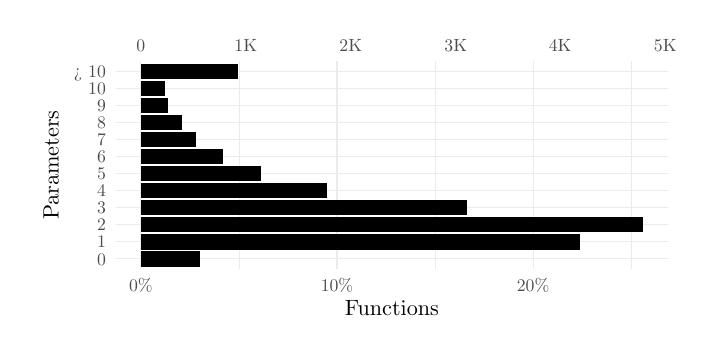
\begin{tikzpicture}[x=1pt,y=1pt]
\definecolor{fillColor}{RGB}{255,255,255}
\path[use as bounding box,fill=fillColor,fill opacity=0.00] (0,0) rectangle (238.49,108.41);
\begin{scope}
\path[clip] ( 31.86, 21.16) rectangle (231.38, 96.31);
\definecolor{drawColor}{gray}{0.92}

\path[draw=drawColor,line width= 0.2pt,line join=round] ( 76.35, 21.16) --
	( 76.35, 96.31);

\path[draw=drawColor,line width= 0.2pt,line join=round] (147.19, 21.16) --
	(147.19, 96.31);

\path[draw=drawColor,line width= 0.2pt,line join=round] (218.04, 21.16) --
	(218.04, 96.31);

\path[draw=drawColor,line width= 0.4pt,line join=round] ( 31.86, 24.86) --
	(231.38, 24.86);

\path[draw=drawColor,line width= 0.4pt,line join=round] ( 31.86, 31.02) --
	(231.38, 31.02);

\path[draw=drawColor,line width= 0.4pt,line join=round] ( 31.86, 37.18) --
	(231.38, 37.18);

\path[draw=drawColor,line width= 0.4pt,line join=round] ( 31.86, 43.34) --
	(231.38, 43.34);

\path[draw=drawColor,line width= 0.4pt,line join=round] ( 31.86, 49.50) --
	(231.38, 49.50);

\path[draw=drawColor,line width= 0.4pt,line join=round] ( 31.86, 55.66) --
	(231.38, 55.66);

\path[draw=drawColor,line width= 0.4pt,line join=round] ( 31.86, 61.81) --
	(231.38, 61.81);

\path[draw=drawColor,line width= 0.4pt,line join=round] ( 31.86, 67.97) --
	(231.38, 67.97);

\path[draw=drawColor,line width= 0.4pt,line join=round] ( 31.86, 74.13) --
	(231.38, 74.13);

\path[draw=drawColor,line width= 0.4pt,line join=round] ( 31.86, 80.29) --
	(231.38, 80.29);

\path[draw=drawColor,line width= 0.4pt,line join=round] ( 31.86, 86.45) --
	(231.38, 86.45);

\path[draw=drawColor,line width= 0.4pt,line join=round] ( 31.86, 92.61) --
	(231.38, 92.61);

\path[draw=drawColor,line width= 0.4pt,line join=round] ( 40.93, 21.16) --
	( 40.93, 96.31);

\path[draw=drawColor,line width= 0.4pt,line join=round] (111.77, 21.16) --
	(111.77, 96.31);

\path[draw=drawColor,line width= 0.4pt,line join=round] (182.62, 21.16) --
	(182.62, 96.31);
\definecolor{fillColor}{RGB}{0,0,0}

\path[fill=fillColor] ( 40.93, 89.84) rectangle ( 76.18, 95.38);

\path[fill=fillColor] ( 40.93, 22.09) rectangle ( 62.34, 27.63);

\path[fill=fillColor] ( 40.93, 28.25) rectangle (199.57, 33.79);

\path[fill=fillColor] ( 40.93, 83.68) rectangle ( 49.80, 89.22);

\path[fill=fillColor] ( 40.93, 34.41) rectangle (222.31, 39.95);

\path[fill=fillColor] ( 40.93, 40.56) rectangle (158.76, 46.11);

\path[fill=fillColor] ( 40.93, 46.72) rectangle (108.20, 52.27);

\path[fill=fillColor] ( 40.93, 52.88) rectangle ( 84.25, 58.43);

\path[fill=fillColor] ( 40.93, 59.04) rectangle ( 70.64, 64.59);

\path[fill=fillColor] ( 40.93, 65.20) rectangle ( 60.94, 70.75);

\path[fill=fillColor] ( 40.93, 71.36) rectangle ( 55.94, 76.91);

\path[fill=fillColor] ( 40.93, 77.52) rectangle ( 50.67, 83.06);
\end{scope}
\begin{scope}
\path[clip] (  0.00,  0.00) rectangle (238.49,108.41);
\definecolor{drawColor}{gray}{0.30}

\node[text=drawColor,anchor=base,inner sep=0pt, outer sep=0pt, scale=  0.64] at ( 40.85, 99.91) {0};

\node[text=drawColor,anchor=base,inner sep=0pt, outer sep=0pt, scale=  0.64] at ( 78.80, 99.91) {1K};

\node[text=drawColor,anchor=base,inner sep=0pt, outer sep=0pt, scale=  0.64] at (116.74, 99.91) {2K};

\node[text=drawColor,anchor=base,inner sep=0pt, outer sep=0pt, scale=  0.64] at (154.69, 99.91) {3K};

\node[text=drawColor,anchor=base,inner sep=0pt, outer sep=0pt, scale=  0.64] at (192.43, 99.91) {4K};

\node[text=drawColor,anchor=base,inner sep=0pt, outer sep=0pt, scale=  0.64] at (230.38, 99.91) {5K};
\end{scope}
\begin{scope}
\path[clip] (  0.00,  0.00) rectangle (238.49,108.41);
\definecolor{drawColor}{gray}{0.30}

\node[text=drawColor,anchor=base east,inner sep=0pt, outer sep=0pt, scale=  0.64] at ( 28.26, 22.65) {0};

\node[text=drawColor,anchor=base east,inner sep=0pt, outer sep=0pt, scale=  0.64] at ( 28.26, 28.81) {1};

\node[text=drawColor,anchor=base east,inner sep=0pt, outer sep=0pt, scale=  0.64] at ( 28.26, 34.97) {2};

\node[text=drawColor,anchor=base east,inner sep=0pt, outer sep=0pt, scale=  0.64] at ( 28.26, 41.13) {3};

\node[text=drawColor,anchor=base east,inner sep=0pt, outer sep=0pt, scale=  0.64] at ( 28.26, 47.29) {4};

\node[text=drawColor,anchor=base east,inner sep=0pt, outer sep=0pt, scale=  0.64] at ( 28.26, 53.45) {5};

\node[text=drawColor,anchor=base east,inner sep=0pt, outer sep=0pt, scale=  0.64] at ( 28.26, 59.61) {6};

\node[text=drawColor,anchor=base east,inner sep=0pt, outer sep=0pt, scale=  0.64] at ( 28.26, 65.77) {7};

\node[text=drawColor,anchor=base east,inner sep=0pt, outer sep=0pt, scale=  0.64] at ( 28.26, 71.93) {8};

\node[text=drawColor,anchor=base east,inner sep=0pt, outer sep=0pt, scale=  0.64] at ( 28.26, 78.09) {9};

\node[text=drawColor,anchor=base east,inner sep=0pt, outer sep=0pt, scale=  0.64] at ( 28.26, 84.25) {10};

\node[text=drawColor,anchor=base east,inner sep=0pt, outer sep=0pt, scale=  0.64] at ( 28.26, 90.41) {> 10};
\end{scope}
\begin{scope}
\path[clip] (  0.00,  0.00) rectangle (238.49,108.41);
\definecolor{drawColor}{gray}{0.30}

\node[text=drawColor,anchor=base,inner sep=0pt, outer sep=0pt, scale=  0.64] at ( 40.93, 13.15) {0{\%}};

\node[text=drawColor,anchor=base,inner sep=0pt, outer sep=0pt, scale=  0.64] at (111.77, 13.15) {10{\%}};

\node[text=drawColor,anchor=base,inner sep=0pt, outer sep=0pt, scale=  0.64] at (182.62, 13.15) {20{\%}};
\end{scope}
\begin{scope}
\path[clip] (  0.00,  0.00) rectangle (238.49,108.41);
\definecolor{drawColor}{RGB}{0,0,0}

\node[text=drawColor,anchor=base,inner sep=0pt, outer sep=0pt, scale=  0.80] at (131.62,  4.40) {Functions};
\end{scope}
\begin{scope}
\path[clip] (  0.00,  0.00) rectangle (238.49,108.41);
\definecolor{drawColor}{RGB}{0,0,0}

\node[text=drawColor,rotate= 90.00,anchor=base,inner sep=0pt, outer sep=0pt, scale=  0.80] at ( 11.20, 58.73) {Parameters};
\end{scope}
\end{tikzpicture}
